\updatehighlight{
    name=accentB,
    add={\tableofcontents}
}

\begin{saveblock}{tableOfContents}
    \begin{highlightblock}[linewidth=0.5\textwidth,gobble=8]
        \begin{document}
            \maketitle
            \tableofcontents

            \section{AA}
            ...
        \end{document}
        ~~
        ~~
        ~~
        ~~
        ~~
        ~~
        ~~
        ~~
    \end{highlightblock}
\end{saveblock}

\addtorecentlist{\textbackslash tableofcontents}

\begin{frame}
    \frametitle{\lang,Contents,Inhoudsopgave,}
    
    \begin{columns}
        \begin{column}{0.5\textwidth}
            \useblock{tableOfContents}
        \end{column}
        \begin{column}{0.5\textwidth}
            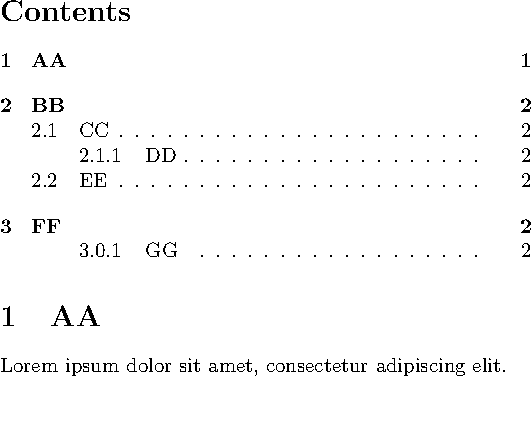
\includegraphics[width=\linewidth,height=0.8\textheight,keepaspectratio,page=1]{assets/tableofcontents.pdf}
        \end{column}
    \end{columns}
\end{frame}

\updatehighlight{
    name=accentB,
    remove={\tableofcontents},
    add={\newpage},
    %
    name=default,
    add={\tableofcontents}
}

\begin{saveblock}{tableOfContents}
    \begin{highlightblock}[linewidth=0.5\textwidth,gobble=8]
        \begin{document}
            \maketitle
            \tableofcontents
            \newpage
            
            \section{AA}
            ...
        \end{document}
            ~~
            ~~
            ~~
            ~~
            ~~
            ~~
            ~~
    \end{highlightblock}
\end{saveblock}

\addtorecentlist{\textbackslash newpage}
\begin{frame}
    \frametitle{\lang,Contents,Inhoudsopgave,}
    
    \begin{columns}
        \begin{column}{0.5\textwidth}
            \useblock{tableOfContents}
        \end{column}
        \begin{column}{0.5\textwidth}
            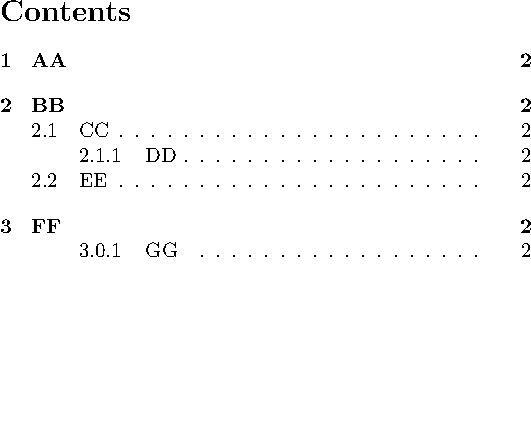
\includegraphics[width=\linewidth,height=0.8\textheight,keepaspectratio,page=1]{assets/tableofcontentswholepage.pdf}
        \end{column}
    \end{columns}
\end{frame}

\updatehighlight{
    name=accentB,
    remove={\newpage},
    add={babel,dutch},
    %
    name=default,
    add={\newpage}
}

\begin{saveblock}{tableOfContents}
    \begin{highlightblock}[linewidth=0.5\textwidth,gobble=8]
        ...
        \usepackage[dutch]{babel}
        
        \begin{document}
            \maketitle
            \tableofcontents
            \newpage
            
            \section{AA}
            ...
        \end{document}
        ~~
        ~~
        ~~
        ~~
    \end{highlightblock}
\end{saveblock}

\addtorecentlist{babel}

\begin{frame}
    \frametitle{\lang,Contents,Inhoudsopgave,}
    
    \begin{columns}
        \begin{column}{0.5\textwidth}
            \useblock{tableOfContents}
        \end{column}
        \begin{column}{0.5\textwidth}
            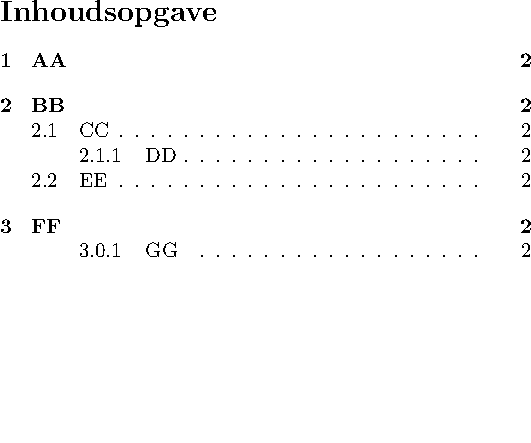
\includegraphics[width=\linewidth,height=0.8\textheight,keepaspectratio,page=1]{assets/tableofcontentsdutch.pdf}
        \end{column}
    \end{columns}
\end{frame}

\updatehighlight{
    name=accentB,
    remove={babel,dutch},
}
